\subsubsection{Implementation of CUDA abstractions}

We assume that we have a fictitious \textbf{Streaming Multiprocessor (SM) core} (Figure \ref{fig: A sub-core of the NVIDIA V100 Streaming Multiprocessor (SM) architecture} page \pageref{fig: A sub-core of the NVIDIA V100 Streaming Multiprocessor (SM) architecture}, same as NVIDIA V100, page \pageref{subsubsection: NVIDIA V100 Streaming Multiprocessor (SM)}) with only \textbf{four warps} of parallel execution in hardware. So there are 4 warps times 32 threads, and \textbf{128 threads} can be executed in parallel each time.

\begin{figure}[!htp]
    \centering
    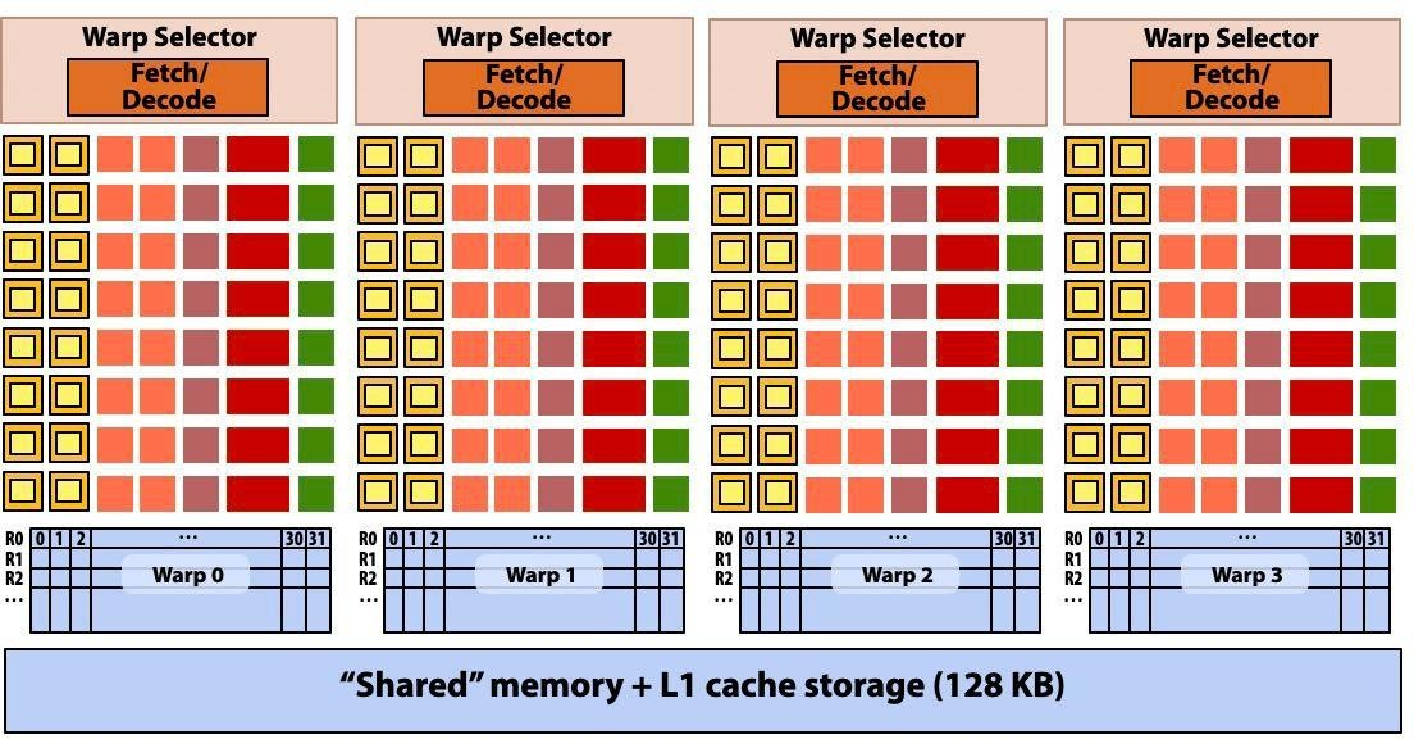
\includegraphics[width=\textwidth]{img/cuda-abs-1.pdf}
    \caption{Streaming Multiprocessor (SM) core, with 4 warps and 128 threads in total.}
\end{figure}

\begin{flushleft}
    \textcolor{Green3}{\faIcon{question-circle} \textbf{Why allocating all threads in a block might be inefficient}}
\end{flushleft}
Now imagine we want to run a CUDA program where a thread \textbf{block} consists of \textbf{256 CUDA threads}, even though our GPU architecture can \emph{only} execute 128 threads at a time. A naive implementation might execute the entire CUDA block by executing four warps (threads 0-127) to completion, and then execute the next four warps (threads 128-255) to completion. This \textbf{sequential execution of warps can lead to inefficiencies} because \textbf{there may be idle periods where some warps are stalled waiting for memory accesses or synchronization points}.

\highspace
\begin{flushleft}
    \textcolor{Green3}{\faIcon{check-circle} \textbf{Use interleaving execution}}
\end{flushleft}
A good alternative is to use interleaved execution. \definition{Interleaved execution} means that the \textbf{GPU schedules warps so that they overlap}. While some warps are waiting for memory access or synchronization, \textbf{others can execute}. This overlapping helps to \textbf{hide latencies} and \textbf{keep the GPU cores busy}.

\highspace
However, \textbf{CUDA kernels can create dependencies between threads in a block}. To manage these dependencies, the programmer can use the function \texttt{\_\_syncthreads()} to synchronize threads within a block. \texttt{\_\_syncthreads()} ensures that \textbf{all threads in the block reach the synchronization point before any thread can continue}. This means that threads 128-255 cannot continue until threads 0-127 reach the synchronization point.

\highspace
\begin{flushleft}
    \textcolor{Green3}{\faIcon{check-circle} \textbf{Why interleaving execution is optimal when there are dependencies}}
\end{flushleft}
If we run four warps to completion before starting the next four, we \textbf{may not be using shared resources} (such as shared memory and execution units) efficiently. This can also \textbf{lead to scenarios where some warps are stalled indefinitely waiting for other warps to reach synchronization points}, causing potential \textbf{\underline{deadlocks}} or inefficiencies.

By interleaving the execution of warps, the GPU can better manage thread dependencies, hide latencies, and make more efficient use of its resources.

\highspace
\begin{lstlisting}[language=C++]
#define THREADS_PER_BLK 256

__global__ void convolve(int N, float* input, float* output)
{
    __shared__ float support[THREADS_PER_BLK * 2];
    int index = blockIdx.x * blockDim.x + threadIdx.x;

    support[threadIdx.x] = input[index];
    if (threadIdx.x < N) {
        support[
            THREADS_PER_BLK + threadIdx.x
        ] = input[index + THREADS_PER_BLK];
    }

    __syncthreads();

    float result = 0.0f; // thread-local
    for (int i = 0; i < 5; i++)
        result += support[threadIdx.x + i];

    output[index] = result;
}
\end{lstlisting}

\begin{flushleft}
    \textcolor{Red2}{\faIcon{book} \textbf{Summary}}
\end{flushleft}
\begin{enumerate}
    \item Thread \textbf{blocks} can be \textbf{scheduled in any order by the system}.
    \begin{itemize}
        \item The system assumes no dependencies between blocks.
        \item Blocks are logically concurrent, similar to ISPC tasks (Implicit SPMD Program Compiler, page \pageref{definitionbox: Implicit SPMD Program Compiler (ISPC)}).
    \end{itemize}

    \item \textbf{CUDA threads in the same block run concurrently} (live at the same time).
    \begin{itemize}
        \item When a block begins executing, all threads exist and have register state allocated.
        \item A \textbf{CUDA thread block is an SPMD} (Single Program, Multiple Data) \textbf{program}, similar to an ISPC gang of program instances.
        \item Threads in a thread block are concurrent, cooperating \dquotes{workers}.
    \end{itemize}

    \newpage

    \item \textbf{CUDA implementation}.
    \begin{itemize}
        \item An NVIDIA GPU warp has performance characteristics \emph{similar} to an ISPC gang of instances.
        \item All warps in a thread block are scheduled onto the same SM (Streaming Multiprocessor), allowing for high-bandwidth, low-latency communication through shared memory variables.
        \item When all threads in a block complete, block resources (shared memory allocations, warp execution contexts) become available for the next block.
    \end{itemize}
\end{enumerate}
 